%!TEX root = main.tex

%%%%%%% SECTION %%%%%%%
\section{Modèle événementiel pour l'intégration du domaine 3D dans les 
EVC}
\label{sec:modele_event}
%\subsection{Introduction}
La méthodologie orientée événements intègre plusieurs aspects souvent laissés 
de côté dans la littérature concernant le développement des environnements 
virtuels collaboratifs pour la visualisation et la manipulation d'objets \gls{3D}. 
Les événements peuvent, en effet, être utilisés dans le cadre de \gls{CSCW} et 
d'\gls{EVC}, qui ont évolué du simple collecticiel à de plus importantes 
organisations virtuelles comme on peut en retrouver dans des environnements 
scientifiques et d'ingénierie. L'idée de partager des ressources communes pour 
travailler sur un projet commun nécessite des outils propres qui implémentent 
des modèles de collaborations adaptés aux fonctionnalités spécifiques des 
systèmes distribués (forums, chats, tableaux blancs partagés \dots). Ces 
collaborations sont routinières, les motifs de collaboration sont bien connus. Les 
motifs consistent en des segments de collaborations récurrents qui peuvent être 
capturés, encapsulés dans des composants distincts et réutilisés comme des 
solutions pour d'autres problèmes liés à la collaboration. Par exemple, les services 
de sensibilisation permettent de traiter les événements et de donner des 
informations à propos du travail collaboratif. En utilisant les événements suivis, 
les services d'analyse fournissent des statistiques à propos des collaborations 
passées et présentes.


Les \gls{EDA} sont par nature des systèmes très peu couplés. Dès lors, les 
données produites lors de la collaboration peuvent facilement être réutilisées pour 
un traitement secondaire comme la sensibilisation aux éléments de 
l'environnement. 
Le découpage de la modélisation logicielle et l'abstraction que le système apporte 
sont aussi l'occasion de s'intéresser à la façon dont sont générées les données 
produites par les utilisateurs et la façon dont elles sont validées, stockées puis 
affichées par le système. 

L'\gls{EP} est à la base de nombreuses applications informatiques dans les domaines de l'énergie, la santé, l'environnement, les transports, la finance, les services et l'industrie. L'\gls{EP} réunit des méthodes et des outils 
pour filtrer, transformer et détecter des motifs dans des événements, dans le but 
de réagir à des conditions qui changent, généralement liées à des contraintes de 
temps \cite{Chandy2011}. L'\gls{EP} intègre plusieurs fonctionnalités pour :
\begin{itemize}
	\item obtenir des données à partir de plusieurs sources en quasi temps réel ;
	\item agréger et analyser ces données pour détecter des motifs qui indiquent la 
	présence de situations critiques qui nécessitent une réponse ;
	\item déterminer la réponse la plus adaptée à ces situations ;
	\item et surveiller (\textit{monitor}) l'exécution de cette réponse.
\end{itemize}

L'\gls{EP} est devenu un paradigme de choix pour les applications proposant des 
outils de surveillance et des applications réactives \cite{Hinze2009}. La 
compréhension des événements à travers leur composition, leur abstraction, leur 
type de traitement et la qualité de service offre un large panorama de domaines 
d'applications et de technologies possibles. 

C'est pourquoi il est nécessaire de définir un cadre à la modélisation 
événementielle : une spécification générique des événements, la définition des 
événements propres à la modélisation 3D collaborative. 
La validation des règles métiers doit également être introduite dans 
le processus de traitement des événements. La visualisation des événements doit 
être assez flexible pour gérer l'arriver des flux d'événements produits ou issus 
de l'intergiciel \gls{P2P} orienté messages (type \gls{PubSub}) par lequel les 
pairs se transmettent les notifications d'événement.



%L'intégration de la partie métier L'un des aspects principaux a été de 
%combiner tous les aspects reliés aux événements dans le \textit{pipeline} de 
%visualisation et de manipulation d'objets 3D. 


\subsubsection{Constat}

Par nature, une \gls{EDA} est extrêmement peu couplée et 
hautement distribuée. Le créateur de l'événement sait seulement que l'événement 
se produit et n'a aucune idée du traitement que l'événement va subir par 
la suite ou de qui cela va concerner. 
C'est pourquoi les \glspl{EDA} sont plus utilisées dans un 
contexte de flux d'information asynchrone. La traçabilité dans ces environnements 
devient alors un enjeu important. Facilitée par l'empreinte laissée par chaque 
événement, elle n'en demeure pas moins complexe selon l'échelle d'évaluation. À 
l'échelle d'un utilisateur, d'un groupe d'utilisateurs ou de plusieurs groupes, les
acteurs restent des entités assez homogènes dans le cadre de la modélisation 
\gls{3D} collaborative ce qui simplifie la tâche car le contexte et le domaine sont
connus.



%Il existe différents types de traitements d'événements : simple, en continu, 
%complexe. 
%Ils peuvent être utilisés ensemble dans le cadre d'une même application.
%\begin{itemize}
%\item Traitement d'événement simple. (\textit{simple event processing}). 
%Dans le traitement simple d'événements, un événement notable arrive, initiant 
%une 
%cascade d'actions. Le traitement simple d'événements est généralement utilisé 
%pour 
%orienter un flux temps-réel qui peut prendre un peu de temps, n'entraînant pas de 
%coût sur la partie métier.
%\item Traitement de flux continus d'événements. (\textit{stream event 
%processing}). 
%\item Traitement d'événements complexes. (\textit{complex event 
%processing}). 
%
%\end{itemize}

Le choix de baser la gestion des données sur le patron de conception \gls{CQRS}, 
combiné à celui de l'\gls{ES}, repose sur le constat suivant : dans un cadre industriel, le 
besoin de traçabilité de l'information est très important, pour suivre l'évolution d'un 
projet par exemple. 
Les \glspl{EDA} reposent le plus souvent sur 
la communication client-serveur pour faciliter la gestion des données dans le 
système distribué. C'est pourquoi l'exploitation du patron de conception 
\gls{CQRS} est traditionnellement développée sur la base d'une architecture client-serveur (pour récupérer les mises à jour). 
Ce fonctionnement ne permet pas le travail hors ligne.

Côté serveur, le stockage des données est de moins en moins cher : il est possible de 
stocker beaucoup de données de manière distante notamment 
grâce l'infonuagique. Le serveur a une puissance de calcul plus importante (et surtout ajustable).

Côté client, la puissance de calcul des machines sur lesquelles sont installés les 
navigateurs web évolue rapidement (notamment les appareils mobiles comme les 
\textit{smartphones} et les tablettes). Les navigateurs suivent cette tendance en 
puisant dans ces ressources (CPU et GPU) pour effectuer des traitements similaires à ceux que 
l'on trouve traditionnellement côté serveur et pour proposer des fonctionnalités 
avancées, telles que le stockage de données sur le client (IndexedDB, 
storageAPI), l'affichage \gls{3D} (WebGL) et la communication en 
\gls{P2P} 
(\gls{WebRTC}). En déportant ainsi la charge que pourrait subir une architecture 
client-serveur côté client, les échanges réseaux sont limités car ils 
sont très coûteux d'un point de vue énergétique pour les appareils mobiles 
\cite{Koskela2015}. De plus, l'utilisation de la bande passante est onéreuse et 
parfois limitée - voire inexistante ; il est donc nécessaire de tirer parti de tous les 
appareils participant à la collaboration, au lieu de tout faire reposer sur le serveur. 
Chaque appareil participant à la collaboration doit être autonome et le plus 
indépendant possible en termes de ressources (données, réseaux, validation 
experte). 

\paragraph{Contribution}
Plusieurs aspects de la contribution dans le modèle événementiel sont décrites ci-après. 
Tout d'abord, il est nécessaire de spécifier les événements qui vont être utilisés
sous une forme générique. Ces événements, qui représentent ce qui se passe dans l'application, 
doivent faire ressortir l'expertise de chaque modification. Que ce soit le contexte 
auquel il est lié, les paramètres qu'il inclus, le type représenté, les informations de chaque événement
sont issues du domaine de la modélisation 3D. 
Puis, le modèle événementiel propose d'adapter les patrons de conception 
\gls{ES} et \gls{CQRS} sous un angle nouveau.
En déportant ces patrons en totalité sur le client, le système est capable de traiter 
le cycle des données de manière autonome (sauf la sauvegarde à long terme) en profitant des
ressources que le client met à disposition. La conservation de la séparation du traitement 
en écriture et en lecture permet au système d'être capable de vérifier la validité des 
modifications entrantes par lui-même et d'être flexible sur les flux sortants d'événements qu'il propose.
Cela simplifie notamment la transmission des données liées à la \gls{3D} et à la collaboration en limitant le 
nombre de requêtes et la taille des données transmises, sans perdre la traçabilité de 
celles-ci. L'idée est de profiter de la puissance du client pour créer une 
architecture assurant l'autonomie de l'utilisateur en cas de déconnexion volontaire 
(travail hors ligne) ou involontaire (coupure). L'utilisateur a la garantie d'avoir 
un historique performant qui profite de chaque connexion au réseau  pour mettre à jour le système.
Le modèle événementiel présenté dans cette thèse inclut également un modèle de cohérence allégé 
Il prend la forme d'un module de détection de conflit basé sur le journal d'événements dont chaque 
client possède une réplique locale.

\subsection{Modèle général}
%TODO
%La composition de l'architecture s'est effectuée, avec en arrière pensée, les lignes 
%directrices  énoncées plus haut\info{ref section} \cite{Xhafa2010}. 
%\todo{reprendre 
%la partie virtualisation dans la partie P2P}


La mise en place d'une \gls{EDA} pour faire de la modélisation \gls{3D} engendre 
des avantages pour tous les métiers engagés (utilisateurs, développeurs, 
analystes métier).
D'une part, la sensibilisation à l'historique des données et aux interactions 
inter-utilisateurs est partagée par les collaborateurs et les analystes métier. 
Les utilisateurs sont mieux informés de l'impact de leurs modifications et 
ont un aperçu général de l'évolution de la scène. D'autre part, 
la sensibilisation à la distribution des données est une composante 
importante pour les utilisateurs et les développeurs. En effet, la répartition 
de la charge permet de profiter du potentiel de calcul de toutes les parties 
prenantes du réseau. 

Dans 3DEvent, le langage partagé se réfère au domaine de la manipulation 
d'objets \gls{3D}, mais aussi à celui de la collaboration. Par exemple, le terme 
de maillage peut se référer à la fois au maillage géométrique ou bien au maillage 
de l'architecture réseau, d'où l'importance de définir les différents contextes en 
amont. 
Notons que le contexte de l'application peut faire varier les frontières d'un 
domaine. Dans cette thèse le contexte est l'assemblage d'objets 3D dans une 
scène 3D. Le modèle issu du domaine défini permet de mettre en valeur les 
aspects métiers liés à l'application.

\subsubsection{Spécification des événements dans le framework}
Le \gls{framework} étant orienté événements, cette section introduit la 
représentation et le vocabulaire utilisé dans la description des événements de 
3DEvent. 3DEvent reprend la représentation proposée par Tominski 
\cite{Doktor-ingenieur2006} illustrée par la Figure \ref{fig:representation_event}. 
Une partie de la contribution est d'adapter les propriétés de cette spécification pour 
la modélisation \gls{3D} collaborative (visualisation et manipulation). 

\begin{figure}[ht]
	\centering
	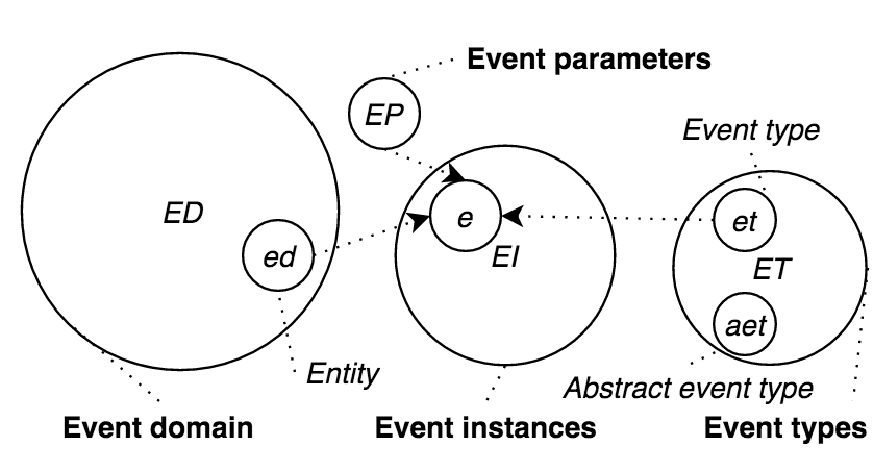
\includegraphics[width=0.7\columnwidth]{eps/event4.eps}
	\caption{Illustration des notions d'événements du domaine, des types 
		d'événements, et des instances d'événements.}
	\label{fig:representation_event}
\end{figure} 

Pour décrire le cadre de référence dans lequel les événements se produisent, la 
notion de domaines d'événements est introduite. Un domaine d'événements 
\textit{ED} (\textit{Event Domain}) contient les événements qui respectent les 
types d'événements spécifiés. Par analogie avec le \gls{DDD}, cet 
espace correspond au contexte borné (cadre d'action) d'un agrégat. À un agrégat, 
sont associés des types d'événements \textit{ET} (\textit{Event Type}) particuliers. 
Un \textit{ET} est utilisé pour exprimer un intérêt concret envers les entités d'un 
\textit{ED}. 
Les événements abstraits \textit{aet} (\textit{abstract event type}) sont 
compatibles avec l'\textit{ED}. 
Une instance d'événements \textit{e} -- ou simplement 
événements -- est composée du triplet \textit{ED}, \textit{ET} et \textit{EP}. 
L'ensemble de toutes les instances d'événements possibles est exprimé par 
\textit{EI}. \textit{EP} (Event Parameters) correspond à l'ensemble des paramètres 
que peut avoir l'\textit{EI}. Ainsi, tous les événements sont liés aux intérêts 
d'un~\textit{ED}. La spécification des événements nécessite de 
s'intéresser à tous les types d'événements qui sont utilisés lors de la manipulation 
et la visualisation d'objets \gls{3D} dans un \gls{EVC}. La détection d'événements 
est un processus qui permet de récupérer les instances d'événements d'un 
\textit{ET} en particulier. Cela peut être utilisé pour la visualisation de types
particuliers par exemple. Dans 3DEvent, la spécification des événements est 
calquée sur les comportements observés lors des expérimentations des premiers 
travaux \cite{Desprat2015a, Desprat2015b}. 

Le Tableau \ref{tab:extraitevent} présente les événements de l'agrégat Maillage -- 
extrait du Tableau \ref{tab:events} qui résume les différents types d'événements 
de base construits à partir du \gls{framework} et les agrégats auxquels ils sont 
associés. Parmi ces événements, l'événement 
\textit{meshAdded} et \textit{meshDropped} semblent très proches, voire 
identiques quant au résultat que l'utilisateur peut obtenir. Cependant, la 
sémantique liée à chacun permet de différencier l'intention de l'utilisateur. 
Pour \textit{meshAdded}, l'utilisateur va, en cliquant sur l'item de la bibliothèque, 
voir apparaître un maillage au centre de la scène. 
Concernant \textit{meshDropped}, l'utilisateur effectue un glissé / déposé de l'objet 
depuis la bibliothèque à l'endroit dans l'environnement 3D où il souhaite que l'objet 
soit positionné.



\begin{table}[ht]
	\centering
	\caption{Événements de 
		l'agrégat Maillage (extrait de Tab. \ref{tab:events}) }
	\label{tab:extraitevent}
	\begin{tabular}{lll}
		\toprule
		\textbf{Événement}& \textbf{Dénomination} & \textbf{Description} \\ \midrule
		%\textbf{Agrégat Maillage}  &                      &             \\ \hline
		Maillage ajouté (*)&     meshAdded                 
		&  \begin{tabular}[c]{@{}l@{}} Un maillage a été ajouté dans\\  la Scène à 
			partir d'une géométrie\\ de la 
			bibliothèque \end{tabular}  \\\hline
		Maillage déposé (*) &     meshDropped               
		&      \begin{tabular}[c]{@{}l@{}} Un maillage a été déposé dans 
			\\l'env. 3D de la Scène à 
			partir \\d'une géométrie de la bibliothèque \end{tabular} \\\hline
		Maillage supprimé & meshRemoved       &        \begin{tabular}[c]{@{}l@{}} 
			Un maillage a été 
			supprimé \\de la Scène \end{tabular}      \\\hline
		Maillage translaté &   meshTranslated  	 &    \begin{tabular}[c]{@{}l@{}} Un 
			maillage a 
			subi une translation \\dans la Scène \end{tabular}              \\\hline
		Maillage pivoté &      meshRotated                &    
		\begin{tabular}[c]{@{}l@{}} Un maillage a 
			subi une rotation \\dans la Scène \end{tabular}           \\\hline
		Maillage mis à l'échelle &  meshScaled           &     
		\begin{tabular}[c]{@{}l@{}} Un maillage a 
			subi une homothétie    \\dans la Scène \end{tabular}    \\ \hline
		\bottomrule
	\end{tabular}
\end{table}

Ce tableau permet de donner un exemple qui reprend la description qui vient d'être 
présentée. L'\textit{ED} correspond donc au \og système de modélisation \gls{3D} 
collaborative\fg{}. Dans ce contexte, l'agrégat \og Maillage\fg{} réagit à un 
certain nombre de types d'événements comme \textit{meshAdded}, 
\textit{meshDropped}\dots Les événements typés sont produits par l'agrégat en 
prenant en compte les paramètres nécessaires à leur instanciation. Par exemple, 
la production d'un événement \textit{meshTranslated} prend en paramètres le 
vecteur de translation (x,y,z) et la référence de l'identifiant de la scène à laquelle il 
appartient.


Plus généralement, le domaine est la représentation des objets \gls{3D} d'un point 
de vue expert. Les objets du domaine représentent les données liées aux 
manipulations \gls{3D} sous une forme abstraite (géométrie, position), 
indépendamment des besoins du rendu (lumière, matériau\dots). Le \gls{framework} intègre un 
générateur d'événements pour faciliter l'implantation de nouveaux types 
d'événements au plus proche des besoins des utilisateurs dans une application de 
modélisation \gls{3D} collaborative (appuyant la sémantique des manipulations).


\subsection{Adaptation des patrons \gls{ES} et \gls{CQRS}}
%TODO celle de la validation des 
%commandes


La Figure \ref{fig:cqrs-client} montre le déroulement du cycle des opérations du 
modèle au sein de \gls{CQRS}, de l'action utilisateur à la visualisation de son 
résultat. 
Du côté de la partie écriture (partie supérieure -- \textit{write part}), lorsque 
l'utilisateur déclenche une commande à partir de l'interface, la commande et ses 
paramètres sont récupérés et traités par le domaine pour être validés selon les 
règles métiers exprimées par ce dernier. Si la modification est validée, le domaine 
produit ou modifie l'agrégat concerné. Ces modifications sont converties sous 
forme d'événements. Les événements sont ensuite transmis à l'Event Store où ils 
sont stockés 
avant d'être transférés à l'Event Publisher. L'Event Publisher joue le rôle 
d'interface entre la partie écriture et la partie lecture. 
Il est également responsable de la 
publication des événements sur le bus d'événements, Event Bus, où sont 
accrochées les différentes projections. Les projections sont nourries à partir des 
événements publiés auxquels elles sont abonnées. Enfin, une Vue (composant
inclus dans l'\gls{IU}) récupère les \glspl{DTO}
contenant les mises à jour à partir d'une projection. La mise à jour d'une Vue peut 
se faire de manière passive -- mode \textit{push} -- (ex. : mises à jour liées à la 
visualisation \gls{3D} des modifications des collaborateurs en temps réel) ou 
active -- mode \textit{pull} -- (ex : aller sur une autre scène) selon le contexte.

\begin{figure}[h]
	\centering
	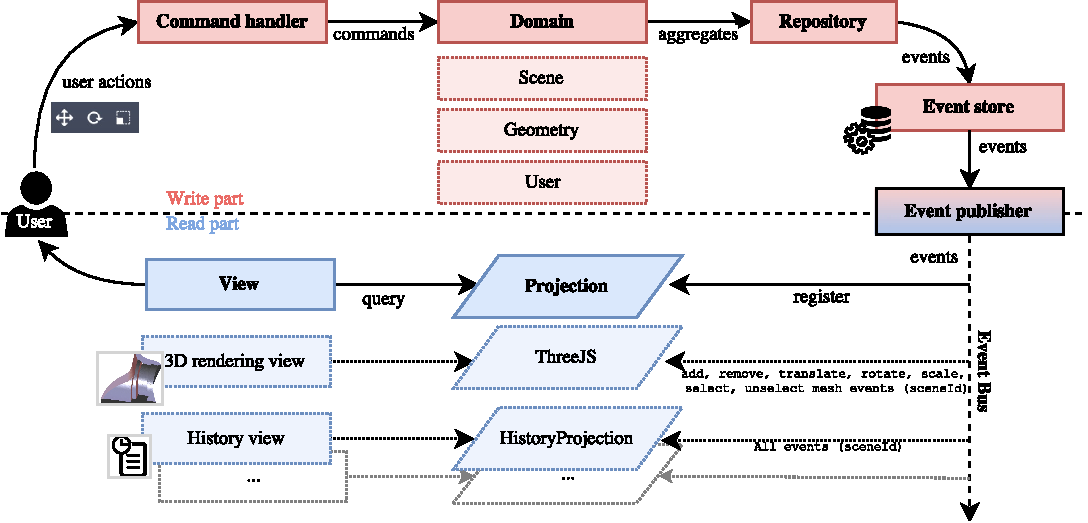
\includegraphics[width=\columnwidth]{eps/cqrs2.pdf}
	\caption[Modèle de l'architecture client dans 3DEvent]{Modèle de l'architecture 
		client dans 3DEvent : la gestion du cycle de vie des données avec 
		\gls{CQRS} 
		et \gls{ES} dans un navigateur web, des actions des utilisateurs à la visualisation 
		en passant par la synchronisation réseau. Issu de \cite{Desprat2017}.}
	\label{fig:cqrs-client}
\end{figure}


Dans ce modèle événementiel, la partie Commande permet de limiter l'introduction 
de données impropres dans le système via différents mécanismes. Chaque 
commande issue de l'\gls{IU} entraîne la génération d'un ou plusieurs événements. 
Ces événements sont considérés 
comme \og soumis\fg{} (\textit{uncommitted}) mais pas encore \og publiés\fg{} 
(\textit{committed}) par le système.
Une commande peut être rejetée pour des raisons variées. Ces raisons sont 
exprimées par différentes phases de validation de la commande.
Une première validation se fait en amont de la création de la commande, avec par 
exemple une vérification de type des paramètres passés à la commande directement
dans l'\gls{IU}.

Le patron \glsreset{ES}\gls{ES} permet de capturer tous les changements d'état 
d'une application sous la forme d'une séquence d'événements. 
Ces événements sont conservés dans un journal et peuvent être 
rejoués pour retrouver l'état de l'application. 
Les événements représentent des faits immuables qui sont ajoutés au journal les
uns après les autres (sans pouvoir en être supprimés), ce qui permet des taux de 
transaction élevés et une réplication efficace (cf. Section \ref{sec:es}). 
Dans 3DEvent, plusieurs composants d'\gls{ES} sont étendus selon 
les applications :

\begin{itemize}
	\item \textit{Acteur.} Un acteur consomme des événements à partir d'un journal 
	d'événements et produit des événements pour le même journal d'événements. 
	L'état interne dérivé à partir des événements consommés est un modèle 
	d'écriture 
	en mémoire (\textit{in-memory}) et contribue à la partie commande (C) du 
	\gls{CQRS}\info{reference à la section}.
	\item \textit{Vue.} Une vue est un acteur qui ne fait que consommer des 
	événements à 
	partir du journal d'événements. L'état interne dérivé à partir des événements 
	consommés est un modèle de lecture en mémoire et contribue à la partie 
	requête (Q) du \gls{CQRS}\info{reference à la section}.
	\item \textit{Producteur.} Un producteur est un acteur qui produit des 
	événements à partir du journal d'événements pour mettre à jour la base 
	de données. L'état interne dérivé à partir des événements consommés est 
	un modèle de lecture en mémoire et 
	contribue à la partie requête (Q) du CQRS (cf. Section \ref{sec:CQRS}).
	\item \textit{Processeur.} Un processeur est un acteur qui consomme des 
	événements à partir d'un journal d'événements et produit les événements 
	traités pour un autre journal d'événements. Les processeurs peuvent être 
	utilisés pour connecter les journaux d'événements au traitement des 
	événements.\info{reference à la section}.
\end{itemize}

%\subsubsection{Collaboration événementielle}

\subsection{Journal des événements}

Les événements produits par un des composants présenté ci-dessus
peuvent être consommés par d'autres de ces composants s'ils partagent un 
journal d'événements local ou distribué. Un journal d'événements (ou Event Store) 
est composé d'agrégats versionnés qui contiennent les instances d'événements 
(Figure \ref{fig:event-store}).
Un journal d'événements peut fonctionner sur un seul site ou être répliqué sur 
plusieurs sites. 
Le site est considéré comme une zone disponible qui accepte 
l'écriture d'un journal d'événements local, même s'il est partitionné sur plusieurs 
sites. Les journaux d'événements locaux, situés sur plusieurs sites, peuvent être 
connectés par le biais d'un journal d'événements dit \og répliqué\fg{} (copié sur une 
autre réplique), qui a pour responsabilité de préserver l'ordre causal des 
événements.

\begin{figure}
	\centering
	\inputTikZ{0.9}{eps/tikz/streams/aggregate.tex}
	\caption{Représentation d'un Event Store stockant des agrégats versionnés qui 
	contiennent des instances d'événements}
	\label{fig:event-store}
\end{figure}

Les sites peuvent être situés à des endroits géographiquement distincts ou sur 
des nœuds à l'intérieur d'une même grappe (\textit{cluster}), ou encore être sur le 
même nœud mais traités séparément selon les zones 
disponibles, qui sont nécessaires au fonctionnement de l'application. 
Les Acteurs et les Processeurs écrivent cependant toujours sur leur journal 
d'événements local. 
Les composants peuvent soit collaborer sur un journal d'événements local sur le 
même site, ou au travers d'un journal répliqué sur différents sites.
Il est important de différencier le journal d'événements de la base de données 
(côté serveur) ; la base de données peut ne contenir qu'une partie du journal. 
Une base de données peut également être considérée comme un élément 
complémentaire au journal d'événements, cependant et bien que parfois 
confondus, ils restent bien distincts conceptuellement.
Le journal d'événements commun est la base des échanges pour communiquer 
par le biais d'événements de collaboration. Ce type d'architecture se retrouve dans 
différents cas d'utilisation :
\improve{est ce que cette section est nécessaire?}
\begin{itemize}
	\item \textit{Processus métier distribués.} Les acteurs de différents types 
	utilisent des événements pour communiquer et parvenir à résoudre un problème 
	commun. Bien qu'ils jouent des rôles différents dans le processus métier, ils 
	réagissent à la réception d'événements (programmation réactive), en 
	mettant à jour l'état de l'application et en produisant de nouveaux événements. 
	Cette forme de collaboration est appelée collaboration dirigée par les 
	événements.\improve{ref}
	\item\textit{Réplication d'état d'Acteur.} Les acteurs de même type consomment 
	les événements de chacun pour répliquer l'état interne avec une cohérence 
	causale. Dans 3DEvent, les opérations concurrentes sont autorisées dans 
	l'environnement pour mettre à jour l'état des acteurs répliqués et permettre la 
	résolution interactive de conflits, en cas de mises à jour concurrentes et 
	conflictuelles. \improve{mieux expliquer}
	\item \textit{Agrégation d'événements.} Les vues et les producteurs agrègent des 
	événements à partir d'autres composants pour générer des vues spécifiques à 
	l'application.
	La collaboration événementielle apporte de la fiabilité quant à la gestion des 
	données dans un système distribué. Par exemple, si un processus distribué 
	échoue à cause d'un problème sur une partie du réseau, le système reprend 
	automatiquement dès que les répliques sont à jour.
\end{itemize}

%\paragraph{Bus d'événement}
Les composants souscrivent à leur journal d'événements en s'accrochant au 
\textbf{bus d'événements}.
Les événements nouveaux sont poussés vers les souscripteurs, 
ce qui leur permet de mettre à jour l'état de l'application avec une latence 
minimale. 
Un événement écrit à un endroit est publié de manière fiable auprès des souscripteurs sur 
ce site et des souscripteurs des sites distants. 
Par conséquent, les composants qui échangent par le biais d'un 
journal d'événements répliqué communiquent via un bus qui préserve l'ordre causal 
des événements de manière durable et tolérant au partitionnement. De ce fait, les 
services sur les partitions du réseau inter-sites (lien entre les sites) peuvent 
continuer à écrire des événements localement. La livraison des événements sur 
les sites distants reprend automatiquement lorsque les partitions sont à jour.


Le journal d'événements est local au site et fournit un ordre total des 
événements stockés. 
Le site est une zone de disponibilité qui héberge un ou plusieurs 
journaux d'événements. Les événements d'un journal d'événements sont 
répliqués sur les sites distants de manière asynchrone. 
Afin de lier des journaux d'événements (localisés sur différents sites) à un journal 
d'événements répliqué, les 
journaux d'événements locaux doivent être accessibles à partir des points 
d'entrées de réplication. De plus, ces points d'entrée doivent être 
connectés entre eux afin de créer un réseau de réplications. 
Un journal d'événements répliqué est représenté par un journal d'événements local 
sur chacun des sites participants.

Les points d'entrée (aussi appelés \glspl{NB})
permettent de gérer un ou plusieurs journaux d'événements. 
Ces journaux sont identifiés pour permettre à la réplication de ne s'intéresser 
qu'aux journaux de même identifiant. 
Les journaux avec différents identifiants sont ainsi isolés les uns des autres et 
leur distribution peut donc varier selon les sites.

Les journaux répliqués fournissent l'ordre causal des événements stockés : l'ordre 
de stockage est le même sur tous les sites, ce qui veut dire que les 
consommateurs qui lisent les événements du journal local vont toujours voir les 
effets avant leurs causes.
\subsection{Flexibilité de la visualisation}
\label{sec:flexviz}
Dans l'approche \gls{CQRS}, une projection est définie comme une dérivation de 
l'état courant à 
partir du flux d'événements. Pour Abdullin, \og la projection est le processus de 
conversion (ou d'agrégation) d'un flux d'événement en une représentation 
structurelle. Cette dernière (qui est mise à jour au moment où le flux est 
parcourue) 
peut avoir différentes appellations : modèle de lecture persistent, vue ou 
état\fg{}\cite{Abdullin2011}.
La partie lecture du modèle (l'affichage sur interface utilisateur) bénéficie des 
projections en lui permettant de réduire l'afflux des événements, ne laissant filtrer 
que ceux qui sont pertinents pour la vue. La projection fournit une vue adaptée 
(filtrée, enrichie\ldots) du flux d'événements au client. Elle peut également être 
utilisée pour mettre en avant des aspects experts (notifications, déclenchement 
d'action) ou des raisons de confidentialité.
Une projection peut être créée de manière synchrone (à la volée) au fur et à 
mesure de la publication des événements ou de manière asynchrone et donc 
découplée du flux des événements. 


Du fait de la nature d'un réseau \gls{P2P}, les pairs ne reçoivent pas forcément les 
paquets réseau de manière ordonnée.
Par conséquent, les messages peuvent arriver dans n'importe quel ordre.
Qu'arriverait-il alors si un événement A ($eA$) nécessitant un autre événement B 
($eB$) arrivait avant celui-ci? Dans cette situation, le système génére une 
erreur en essayant d'appliquer $eA$ sur un état inadéquat car il n'a pas 
d'information sur la hiérarchie d'application des événements ($eB$ puis $eA$).

Pour pallier à ce problème, l'introduction du système de projection permet d'avoir 
un mécanisme (comme un automate fini) qui défini les transitions nécessaires 
pour 
passer d'un état à l'autre. Les transitions réalisent les actions déterminées en 
fonction des 
événements qui arrivent. Par exemple, si un utilisateur essaie d'ajouter un objet 
dans une 
scène  ($eA$) sans avoir créer la scène ($eB$) la projection met en attente $eA$ 
jusqu'à recevoir $eB$. Dans le cas où $eB$ n'arrive jamais, la projection ne pourra 
jamais utiliser $eA$.

\subsection{Cohérence éventuelle en CQRS}


La \gls{CE}, ou \textit{eventual consistency}, propose dans un système 
distribué contenant plusieurs répliques d'avoir une coordination lâche entre ces 
répliques. Cela apporte de nombreux avantages en termes de disponibilité, 
tolérance aux fautes et sécurité des données, et évite l'intégration de protocoles comme \textit{2 
phase commit} ou de protocoles \textit{Paxos} (consensus) complexifiant les échanges. 
La \gls{CE} introduit l'idée que toutes les répliques se réconcilient au bout d'un 
moment (\textit{forward progression}) pour avoir le même état final. Si le caractère 
vicié d'une information est détecté, le système doit le \og réparer\fg{} pour obtenir 
le bon état. 
\begin{figure} [ht]
	\centering
	\inputTikZ{0.6}{eps/tikz/cap.tex}
	\caption{Théorème CAP et les algorithmes de compromis}
	\label{fig:cap}
\end{figure}
L'ordonnancement des événements durant les mises à jour reste identique lorsque
les événements sont rejoués par la suite car l'ordre issu de l'\gls{ES} est 
déterminé par l'ordonnancement des événements stockés 
localement. Au sein d'une réplique, tous les composants \gls{CQRS} respectent 
cet ordonnancement. Les répliques distantes du journal d'événements sont 
cohérentes si les évènements respecte l'ordre causale \cite{Lamport1978} : les 
événements liés causalement ont le même ordre sur tous les sites, alors que les 
événements concurrents peuvent avoir un ordre différent. Cette propriété est 
importante pour obtenir une cohérence causale forte dans une application qui 
respecte le théorème \gls{CAP} (Figure \ref{fig:cap}).  
\blockquote[]{\textit{The largest single benefit about CQRS is when you 
start running into problems with the CAP theorem}}{\cite{Young2010}}.
Young justifie ensuite que le lien entre \gls{CAP} et \gls{CQRS} est plus ténu qu'il 
n'y paraît. Même si \gls{CQRS} ne permet pas d'éviter le dilemme de \gls{CAP}, le 
fait que \gls{CQRS} découpe le système en petites parties permet d'ajuster la 
cohérence séparément.

Dans \gls{CQRS}, l'interaction avec plusieurs agents (utilisateurs, services) est 
découplée et subit un traitement réparti dont résulte la cohérence éventuelle de 
l'application. Dans la conception d'interaction pour l'interface, la synchronicité peut 
varier en fonction certains contextes. 
Les interactions asynchrones rajoutent souvent des étapes qui polluent l'interface.  
Par exemple, dans le cas de l'interaction suivante : \texttt{soumission de 
formulaire -> envoi asynchrone -> message de confirmation}, si l'utilisateur attend 
que la soumission soit une requête qui peut probablement échouer, alors 
l'asynchronisme se justifie pour être capable de fournir une explication à 
l'utilisateur en cas d'erreur. 
La probabilité d'échec peut être réduite en pré-validant la commande. Si personne 
d'autre que l'utilisateur ne travaille sur l'agrégat, la probabilité d'échec est 
quasi-nulle. 
De ce fait, l'asynchronicité rajoute une interaction inutile au flux dans le cas où 
peu de gens travaillent sur la même instance d'agrégat.
Par exemple, il est intéressant de rendre l'exécution d'une commande synchrone 
et la mise à jour de la vue asynchrone. 
Les modèles de cohérence sont des décisions liées au métier car ils ont un 
impact direct sur l'expérience utilisateur. 



L'\gls{ES} donne la possibilité de gérer les conflits liés à la concurrence avec une 
fine granularité. Par exemple, selon le scenario suivant :  $UserA$ a effectué une 
une translation $MeshTrans\-latedEvent$ sur le maillage 
$mesh1$ au moment où $UserB$ a effectué une rotation $MeshRotatedEvent$ sur ce 
même objet. Lors de la sauvegarde des événements, la version de l'agrégat 
$mesh1$ est différente chez chacun des deux utilisateurs. Le module détecteur de conflits 
contient un registre des procédures à suivre en fonction des événements qui sont en conflit entre eux. L'algorithme \ref{algo:conflictregister} 
présente la fonction utilisée pour détecter des conflits dans une liste d'événements donnée. La fonction permet de savoir si un conflit est 
levé à partir de la liste d'événements donnée et du registre des conflits.

\begin{algorithm} % enter the algorithm environment
	\caption{Registre de conflits} % 
	%give the algorithm a caption
	\label{algo:conflictregister} % and a label for \ref{} commands later in the 
	%document
	\begin{algorithmic} % enter the algorithmic environment
		
		\Require $eventToCheck \leftarrow$ list of events to check conflict with\\
		$conflictRegister \leftarrow  Dictionary<Type, List<Type>>$
		\Ensure return true if a conflict is raised
		\Function{ConflictsWith}{$eventToCheck:Type,  previousEvents:List<Type>$}
		%// If type not registered assume the worst and say it conflicts
		\If{$eventToCheck \in conflictRegister$}
		\For{$et \in  previousEvent$}
		\If {$conflictRegister[eventToCheck] == et$}
		\State \Return $true$
		\EndIf
		\EndFor
		\EndIf
		\State \Return $false$
		\EndFunction
	\end{algorithmic}
	
\end{algorithm}


%Linéaire (strong consistency)
%one version replace another -- one parent and one children in the sequence
%each version is immutable 
%each version has an identity
%each new version is a replacement of the previous (earlier)
%directed acyclic graph (eventual consistency)
%each version may have one or more parent
%each parent may have one or more parent
%each parent may have children with different parents
%each version is immutable
%each version has an identity
%
%each version may be viewed as one of many replacement version for its parents
%
%version are immutable and (should) have immutable names


%\begin{algorithm}[caption="titi"]
%	
%    saveEvents(itemId:string, events:EventMessage[], expectedVersion:number) 
%{\\
%    	var eventDescriptors:EventDescriptor[] = 
%this.eventDescriptorsByAggregate[itemId];\\
%    	if (!eventDescriptors) {\\
%    		eventDescriptors = this.eventDescriptorsByAggregate[itemId] = [];\\
%    	} else if (eventDescriptors.length > 0 \&\& 
%eventDescriptors[eventDescriptors.length\\ - 1].version != expectedVersion \&\& 
%expectedVersion != -1) {\\
%    	throw new Error("ConcurrencyException");\\
%    }
%    var i = expectedVersion;\\
%    events.forEach((event:EventMessage) => {\\
%    	i++;\\
%    	event.version = i;\\
%    	var eventDescriptor = {id: event.AggregateId(), version: i, eventData: 
%event};\\
%    	eventDescriptors.push(eventDescriptor);\\
%    	this.\_publisher.publish(event);\\
%    	this.\_network.publishEvent(event);\\
%    });
%}
%\end{algorithm}

%\begin{figure}[htb]
%	\centering
%	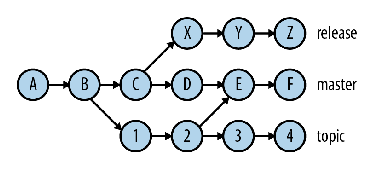
\includegraphics[width=0.3\columnwidth]{gitgraph}
%	\caption{Exemple d'arbre de commits Git}
%	\label{fig:git}
%\end{figure}
\subsection{Bilan}

Le modèle orienté événements pour la modélisation \gls{3D} collaborative, présenté 
dans cette section, intègre les besoins métiers par différents aspects. Le suivi des 
directives liées au \gls{DDD} permet de mieux cerner les règles 
métiers pour les intégrer dans \gls{CQRS}. 

La description de la typologie des événements manipulés insiste sur le compartimentage 
des objets métiers. La modélisation \gls{3D} collaborative est minutieusement étudiée 
pour en dégager les quatre agrégats fondamentaux (la scène, le maillage, la géométrie 
et l'utilisateur) et les types d'événements qui leur sont associés. Cette étape introduit 
des différences fines sur les événements qui sont produits à partir d'un agrégat 
-- un aspect intéressant notamment pour l'observation et la surveillance du contenu 
des sessions collaboratives, développées en Section \ref{sec:flexviz}.
Les composants du patron \gls{CQRS} favorisent le découplage de l'application 
pour obtenir une gestion de la cohérence plus fine. 

La partie \gls{ES} s'intéresse à la sauvegarde des événements dans un journal 
d'événements, et notamment dans le cas des applications distribuées en proposant 
un mécanisme de synchronisation pour détecter les conflits. La fonction principale 
de cette partie est de permettre de recréer un état de l'application cohérent en 
intégrant implicitement une gestion de version des événements.

Ce modèle introduit le cadre de travail pour utilisateur expert en manipulation 
\gls{3D}. Il peut être facilement adapté pour différents types d'applications et étendu à 
d'autres utilisations. 
Pour mettre en avant l'expertise de chacun et profiter de 
toutes les ressources apportées par un utilisateur, une communication efficace de 
ces événements pour la collaboration doit désormais être établie entre les 
collaborateurs.